\section{Ordinal Regression}

\subsection{Recommended References}
\begin{frame}{Recommended References}
	\begin{vfilleditems}
		\item \textcite{gelman2013bayesian} - Chapter 16, Section 16.2: Models for multivariate and multinomial responses
		\item \textcite{mcelreath2020statistical} - Chapter 12, Section 12.3: Ordered categorical outcomes
		\item \textcite{gelman2020regression} - Chapter 15, Section 15.5: Ordered and unordered categorical regression
		\item \textcite{Burkner_Vuorre_2019}
		\item \textcite{Semenova_2019}
	\end{vfilleditems}
\end{frame}

\subsection{What is Ordinal Regression?}
\begin{frame}{What is Ordinal Regression?}
	\textbf{Ordinal regression} is a regression model for \textbf{discrete data} and,
	more specific, when the \textbf{values of the dependent variables have a ``natural ordering''}.
	\vfill
	For example, opinion polls with its plausible ordered values from agree-disagree,
	or a patient perception of pain score.
\end{frame}

\begin{frame}{Why not just use Linear Regression?}
	The main reason to not simply use linear regression with ordinal discrete outcomes is
	that the categories of the dependent variable could not be \textbf{equidistant}.
	This is an assumption in linear regression
	(and in almost all models that use ``metric'' dependent variables):
	the distance between, for example, $2$ and $3$ is not the same distance between $1$ and $2$.
	\vfill
	This assumption can be \textbf{violated in an ordinal regression}.
\end{frame}

\subsection{How to deal with an Ordinal Dependent Variable?}
\begin{frame}{How to deal with an Ordinal Dependent Variable?}
	Surprise! Plot twist!
	\vfill
	Another \textbf{non-linear transformation}.
\end{frame}

\begin{frame}{Cumulative Distribution Function -- CDF}
	In the case of ordinal regression,
	first we need to transform the \textbf{dependent variable into a
		cumulative scale}
	\vfill
	For this, we use the cumulative distribution function (CDF):

	$$P(Y \leq y) = \sum^y_{i=y_{\text{min}}} P(Y = i)$$

	CDF is a \textbf{monotonically increasing function} that represents the
	\textbf{probability of a random variable $Y$ taking values less than
		a certain value $y$}
\end{frame}

\begin{frame}{Log-cumulative-odds}
	Still, this is not enough.
	We need to apply the \textbf{logit function onto the CDF}:

	$$\mathrm{logit}(x) = \mathrm{logistic}^{-1}(x) = \ln\left(\frac{x}{1 -x}\right)$$

	where $\log$ is the natural log function.
	\vfill
	The logit function is the inverse of the logistic function:
	it takes as input any value between $0$ and $1$ (e.g. a probability)
	and outputs an unconstrained real number which we call
	\textbf{logodds}\footnote{we already seen it in logistic regression.}.
	\vfill
	As the transformation is performed onto the CDF,
	we call the result as the CDF logodds or \textbf{log-cumulative-odds}.
\end{frame}

\begin{frame}{$K-1$ Intercepts}
	What do we do with this \textbf{log-cumulative-odds}?
	\vfill
	It allows us to construct \textbf{different intercepts for all possible
		values of the ordinal dependent variable}.
	We create an \textbf{unique intercept for $k \in K$}.
	\vfill
	Actually is $k \in K-1$.
	Notice that the maximum value of the CDF of $Y$ will always be $1$.
	Which translates to a log-cumulative-odds of $\infty$,
	since $p=1$:

	$$\ln \frac{p}{1-p} = \ln \frac{1}{1-1} = \ln 0 = \infty$$

	Hence, we need only \textbf{$K-1$ intercepts for all $K$ possible
		values that $Y$ can take}.
\end{frame}

\begin{frame}{Violation of the Equidistant Assumption}
	Since each intercept implies a different CDF value for each $k \in K$,
	we can safely \textbf{violate the equidistant assumption} which is
	not valid in almost all ordinal variables.
\end{frame}

\begin{frame}{Cut Points}
	Each intercept implies in a log-cumulative-odds for each $k \in K$;
	We need also to \textbf{undo the cumulative nature of the $K-1$ intercepts}.
	Firstly, we \textbf{convert the log-cumulative-odds back to a
		valid probability with the logistic function}:

	$$\mathrm{logit}^{-1}(x) = \mathrm{logistic}(x) = \frac{1}{1 + e^{-x}}$$

	Then, finally, we remove the cumulative nature of the CDF by
	\textbf{subtracting every one of the $k$ cut points by the
		$k-1$ cut point}:
	$$P(Y=k) = P(Y \leq k) - P(Y \leq k-1)$$
\end{frame}

\begin{frame}{Example - Probability Mass Function of an Ordinal Variable}
	\centering
	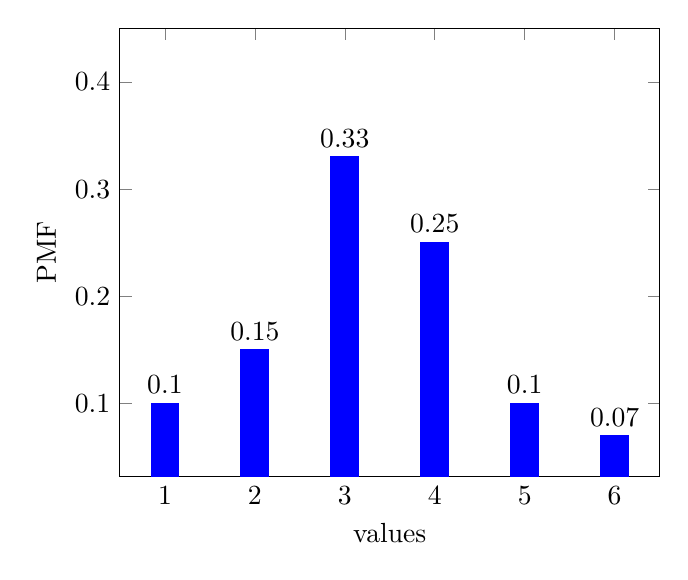
\begin{tikzpicture}[ybar]
		\begin{axis}[
				nodes near coords={\pgfmathprintnumber[fixed,precision=3]{\pgfplotspointmeta}},
				xlabel=values,
				ylabel=PMF,
				xtick={1,2,3,4,5,6},
				ytick={0.1,0.2,0.3,0.4},
				ymax=0.45]
			\addplot [draw=blue, fill=blue] coordinates {
					(1, 0.10)
					(2, 0.15)
					(3, 0.33)
					(4, 0.25)
					(5, 0.10)
					(6, 0.07)
				};
		\end{axis}
	\end{tikzpicture}
\end{frame}

\begin{frame}{Example - CDF versus Log-cumulative-odds}
	\begin{columns}
		\begin{column}{0.5\textwidth}
			\centering
			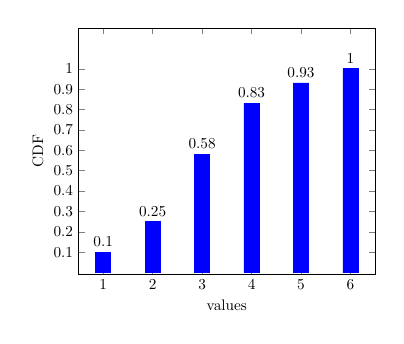
\begin{tikzpicture}[
					ybar,
					scale=0.55]
				\begin{axis}[
						nodes near coords={\pgfmathprintnumber[fixed,precision=3]{\pgfplotspointmeta}},
						xlabel=values,
						ylabel=CDF,
						xtick={1,2,3,4,5,6},
						ytick={0.1,0.2,0.3,0.4,0.5,0.6,0.7,0.8,0.9,1.0},
						ymax=1.2]
					\addplot [draw=blue, fill=blue] coordinates {
							(1, 0.10)
							(2, 0.25)
							(3, 0.58)
							(4, 0.83)
							(5, 0.93)
							(6, 1.00)
						};
				\end{axis}
			\end{tikzpicture}
		\end{column}
		\begin{column}{0.5\textwidth}
			\centering
			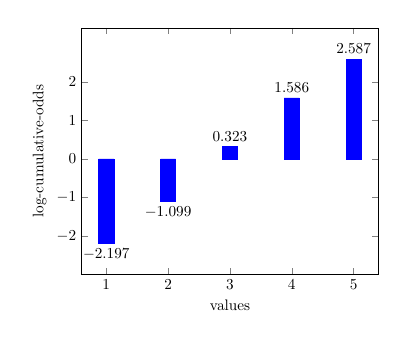
\begin{tikzpicture}[
					ybar,
					scale=0.55]
				\begin{axis}[
						nodes near coords={\pgfmathprintnumber[fixed,precision=3]{\pgfplotspointmeta}},
						xlabel=values,
						ylabel=log-cumulative-odds,
						xtick={1,2,3,4,5,6},
						ytick={-2,-1,0,1,2},
						ymax=3.4,
						ymin=-3]
					\addplot [draw=blue, fill=blue] coordinates {
							(1, -2.19722)
							(2, -1.09861)
							(3, 0.322773)
							(4, 1.58563)
							(5, 2.58669)
							(6, 10.0)
						};
				\end{axis}
			\end{tikzpicture}
		\end{column}
	\end{columns}
\end{frame}

\subsection{Adding Coefficients $\boldsymbol{\beta}$}
\begin{frame}{Adding Coefficients $\boldsymbol{\beta}$}
	With the equidistant assumption solved with $K-1$ intercepts,
	we can add coefficients to represent the independent variable's
	effects into our ordinal regression model.
\end{frame}

\begin{frame}{More Log-cumulative-odds}
	We've transformed all intercepts into log-cumulative-odds so that we
	can add effects as weighted sums of the independent variables to our
	basal rates (intercepts).
	\vfill
	For every $k \in K-1$, we calculate:

	$$\phi_k = \alpha_k + \beta_i x_i$$

	where $\alpha_k$ is the log-cumulative-odds for the $k \in K-1$ intercepts,
	$\beta_i$ is the coefficient for the $i$th independent variable $x_i$.
	\vfill
	Lastly, $\phi_k$ represents the linear predictor for the $k$th intercept.
\end{frame}

\begin{frame}{Matrix Notation}
	This can become more elegant and computationally efficient if we use
	matrix/vector notation:

	$$\boldsymbol{\phi} = \boldsymbol{\alpha} + \mathbf{X} \cdot \boldsymbol{\beta}$$

	where $\boldsymbol{\phi}$, $\boldsymbol{\alpha}$ e
	$\boldsymbol{\beta}$\footnote{
		note that both the coefficients and intercepts will have to be
		interpret as odds, like we did in logistic regression.}
	are vectors and $\mathbf{X}$ is the data matrix,
	in which every line is an observation and every column an independent variable.
\end{frame}

\subsection{Ordinal Regression Specification}
\begin{frame}{Ordinal Regression Specification}
	\footnotesize
	$$
		\begin{aligned}
			\mathbf{y}          & \sim \text{Categorical}(\mathbf{p})                                                \\
			\mathbf{p}          & = \text{logistic}(\boldsymbol{\phi})                                               \\
			\boldsymbol{\phi}   & = \boldsymbol{\alpha} + \mathbf{X} \cdot \boldsymbol{\beta}                        \\
			\alpha_1            & = \text{logit}(\text{CDF}(y_1))                                                    \\
			\alpha_k            & = \text{logit}(\text{CDF}(y_k) - \text{CDF}(y_{k-1})) \text{ for } 2 \leq k \leq K \\
			\alpha_{K}          & = \text{logit}(1 - \text{CDF}(y_{K-1}))                                            \\
			\boldsymbol{\alpha} & \sim \text{Normal}(\mu_\alpha, \sigma_\alpha)                                      \\
			\boldsymbol{\beta}  & \sim \text{Normal}(\mu_{\boldsymbol{\beta}}, \sigma_{\boldsymbol{\beta}})
		\end{aligned}
	$$
	\begin{vfilleditems}
		\footnotesize{
			\item $\mathbf{y}$ -- ordinal discrete dependent variable.
			\item $\mathbf{p}$ -- probability vector of size $K$.
			\item $K$: number of possible values that $\mathbf{y}$ can take, i.e. number of ordered discrete values.
			\item $\boldsymbol{\phi}$: log-cumulative-odds, i.e. the cut points considering the intercepts and the weighted sum of the independent variables.
			\item $\alpha_k$: intercept in log-cumulative-odds for every $k \in K-1$.
			\item $\mathbf{X}$: data matrix of the independent variables.
			\item $\boldsymbol{\beta}$: coefficient vector with size the same as the number of columns of $\mathbf{X}$.
		}
	\end{vfilleditems}
\end{frame}
